\documentclass[11pt,a4paper]{article}

\usepackage[utf8]{inputenc}
\usepackage[T1]{fontenc}
\usepackage[italian]{babel}
\usepackage{amsmath}
\usepackage{amssymb}
\usepackage{graphicx}
\usepackage{booktabs}
\usepackage{geometry}
\usepackage{listings}
\usepackage{xcolor}
\usepackage{hyperref}
\usepackage{caption}

\geometry{margin=2.7cm}

\definecolor{codebg}{rgb}{0.96,0.96,0.96}
\definecolor{codecomment}{rgb}{0.4,0.4,0.4}
\definecolor{codekeyword}{rgb}{0.0,0.0,0.6}

\lstset{
    language=C++,
    backgroundcolor=\color{codebg},
    basicstyle=\ttfamily\footnotesize,
    keywordstyle=\color{codekeyword}\bfseries,
    commentstyle=\color{codecomment}\itshape,
    numbers=left,
    numberstyle=\tiny,
    numbersep=6pt,
    breaklines=true,
    frame=single,
    captionpos=b,
    tabsize=2,
    showstringspaces=false
}

\hypersetup{
    colorlinks=true,
    linkcolor=blue,
    urlcolor=blue,
    citecolor=blue
}

\title{Propagazione parallela di regole logiche pesate su GPU\\
\large Relazione del progetto ArcPal -- Architetture Parallele}
\author{Alessandro Minisini}
\date{\today}

\begin{document}

\maketitle
\tableofcontents

\newpage

\section{Introduzione}

Il progetto ArcPal implementa, in CUDA, un \emph{propagatore parallelo} per un frammento di
linguaggio logico basato su regole pesate. Il problema è quello tipico della propagazione
proposizionale: data una base di regole e un'assegnazione parziale di verità, si vuole estendere
l'assegnazione applicando ripetutamente le regole di inferenza, fino a raggiungere un punto fisso
in cui nessuna ulteriore deduzione è possibile, oppure fino a rilevare una contraddizione.

Il vincolo principale imposto dalla specifica del progetto (riportata nel documento
\texttt{tema.pdf} fornito con l'assegnazione) è che il programma debba scalare con istanze di
dimensione arbitraria, limitate solo dalla memoria disponibile sulla GPU. Questo ha guidato sia la
scelta delle strutture dati (rappresentazioni compatte e contigue, trasferibili in blocco sul
device) sia l'esplorazione di diverse strategie di parallelizzazione, che vanno dal semplice
ri-lancio iterativo di un kernel fino all'uso di \emph{cooperative groups} per realizzare l'intero
ciclo a punto fisso all'interno di un singolo kernel.

Il repository contiene nove implementazioni CUDA distinte dello stesso algoritmo logico,
organizzate in due famiglie (\emph{rule-driven} e \emph{atom-driven}), più una baseline seriale su
CPU usata come riferimento di correttezza. Come caso di studio per il testing su larga scala è
stato usato il Sudoku, le cui celle e vincoli sono codificati come atomi e regole pesate.

Questa relazione descrive: la formalizzazione del problema (Sezione~\ref{sec:problema}); il
formato e la rappresentazione in memoria dei dati di input (Sezione~\ref{sec:dati}); le diverse
strategie di parallelizzazione adottate (Sezione~\ref{sec:strategie}); la metodologia di testing
(Sezione~\ref{sec:testing}); e infine i risultati di performance raccolti sul benchmark Sudoku
(Sezione~\ref{sec:risultati}).

\section{Descrizione del problema}
\label{sec:problema}

\subsection{Regole pesate}

Sia $\mathcal{A}$ un insieme finito di atomi proposizionali. Si considera un frammento di
linguaggio logico costituito da sole regole della forma

\begin{equation}
h \leftrightarrow B \le \{L_1 : w_1, \dots, L_k : w_k\},
\label{eq:rule}
\end{equation}

dove $h$ è la \emph{head} della regola e il \emph{body} viene denotato con
$W \equiv B \le \{L_1:w_1,\dots,L_k:w_k\}$. Sia $h$ che $L_1,\dots,L_k$ sono letterali
proposizionali ground (atomi o loro negazioni), mentre $B$ (il \emph{bound}) e i pesi
$w_1,\dots,w_k$ sono interi positivi.

Dato un insieme di letterali $M$ non contraddittorio, $M$ soddisfa un letterale $L$ ($M \models
L$) se $L \in M$, lo falsifica se $L^c \in M$, altrimenti $L$ è indeterminato. $M$ è completo se
per ogni atomo contiene esattamente uno tra l'atomo e la sua negazione.

Per ogni regola e per un dato $M$ si definiscono le quantità

\[
S_{sat} = \sum_{\substack{i \in \{1,\dots,k\}\\ M \models L_i}} w_i, \qquad
S_{undef} = \sum_{\substack{i \in \{1,\dots,k\}\\ L_i \text{ indeterminato}}} w_i, \qquad
S_{max} = S_{sat} + S_{undef}.
\]

Il body $W$ è vero se $B \le S_{sat}$ (cioè se il peso dei letterali già soddisfatti raggiunge il
bound), e questa nozione è ben definita anche quando alcuni $L_i$ sono ancora indeterminati. $M$
soddisfa la regola $h \leftrightarrow W$ se soddisfa la bi-implicazione.

\subsection{Propagazione}

Dato un insieme $P$ di regole e un'assegnazione (eventualmente parziale) $M$, l'obiettivo è
estendere $M$ sfruttando le regole di $P$, in modo che nessuna regola venga falsificata. Le due
direzioni di propagazione sono:

\begin{description}
\item[Body $\to$ Head.] Se $S_{sat} \ge B$ allora $h$ deve essere posto vero; se $S_{max} < B$
allora $h$ deve essere posto falso. Se $h$ risulta già assegnato al valore complementare si ha una
contraddizione.
\item[Head $\to$ Body.] Se $M \models h$ allora $W$ deve essere soddisfatto: per ogni $L_i$
indeterminato, $L_i$ va propagato (posto vero) esattamente quando $S_{max} - w_i < B$, perché
altrimenti nemmeno rendendo veri tutti gli altri letterali indeterminati si raggiungerebbe il
bound. Simmetricamente, se $M \models h^c$ allora $W$ non può essere soddisfatto: per ogni $L_i$
indeterminato, $L_i^c$ va propagato esattamente quando $S_{sat} + w_i \ge B$, perché altrimenti
rendere vero $L_i$ farebbe superare il bound, violando la regola.
\end{description}

L'inserimento di un nuovo letterale in $M$ può abilitare ulteriori propagazioni: il processo deve
quindi essere iterato fino a un punto fisso, cioè finché non ci sono più variazioni in $M$ oppure
finché non si rileva una contraddizione.

\subsection{Obiettivo del progetto}

Il propagatore CUDA deve calcolare, a partire da $P$ e da un $M$ iniziale parziale, l'estensione
massimale $\hat M$ di $M$ che non falsifica alcuna regola di $P$ (oppure segnalare un fallimento se
tale $\hat M$ non esiste), e classificare ogni regola come soddisfatta, violata o indeterminata
rispetto a $\hat M$. Tutto ciò deve avvenire con un grado di parallelismo che sfrutti la GPU su
istanze di dimensione limitata solo dalla memoria del device.

\section{Rappresentazione e memorizzazione dei dati}
\label{sec:dati}

\subsection{Formato di input testuale}

L'input è un testo in stile DIMACS, letto da standard input dal parser
(\texttt{src/parser.cpp}, dichiarato in \texttt{include/parser.hpp}):

\begin{itemize}
\item una riga \texttt{p <num\_atomi> <num\_regole>} di intestazione;
\item \texttt{num\_regole} righe \texttt{r <head> <bound> <k> <lit$_1$> <w$_1$> \dots\ <lit$_k$> <w$_k$>},
una per regola, dove \texttt{head} è un letterale (positivo = atomo, negativo = sua negazione) e
i \texttt{k} letterali del body sono dati come coppie letterale/peso;
\item una riga \texttt{a <lit\_1> <lit\_2> \dots 0} con l'assegnazione iniziale (i fatti noti),
terminata da \texttt{0}.
\end{itemize}

Ad esempio, il test \texttt{tests/input/test1.in}:

\begin{lstlisting}[language=,basicstyle=\ttfamily\small,frame=single]
p 4 2
r 3 5 2 1 3 -2 4
r -4 2 2 3 2 2 1
a 1 -2 0
\end{lstlisting}

descrive 4 atomi e 2 regole: la regola 0 ha head sull'atomo 3, bound 5 e body
$\{1:3,\, \lnot 2:4\}$; la regola 1 ha head $\lnot 4$, bound 2 e body $\{3:2,\,2:1\}$;
l'assegnazione iniziale pone l'atomo 1 vero e l'atomo 2 falso. Il parser legge i token con
\texttt{cin}, popolando direttamente le strutture descritte di seguito; non viene costruita alcuna
rappresentazione ad albero o a lista delle regole.

\subsection{Struttura \texttt{DIMACSInput}: layout a vettori piatti (CSR)}

Il parser produce la struttura \texttt{DIMACSInput} (\texttt{include/parser.hpp}):

\begin{lstlisting}
enum TruthValue { FALSE = 0, UNDEF = -1, TRUE = 1 };

struct DIMACSInput {
    int num_atoms;
    int num_rules;

    vector<int> M;             // M[0] inutilizzato, M[1..num_atoms]
    vector<int> head;          // head[r] = letterale head della regola r
    vector<int> bound;         // bound[r] = bound B della regola r
    vector<int> rule_offsets;  // offset di inizio body, size = num_rules+1
    vector<int> flat_lits;     // letterali di tutti i body, concatenati
    vector<int> flat_weights;  // pesi corrispondenti a flat_lits
};
\end{lstlisting}

Le regole non sono memorizzate come oggetti separati con un proprio vettore di letterali: i body di
tutte le regole vengono concatenati in due vettori piatti, \texttt{flat\_lits} e
\texttt{flat\_weights}, mentre \texttt{rule\_offsets} indica, per ogni regola, l'intervallo
$[\texttt{rule\_offsets}[r], \texttt{rule\_offsets}[r+1])$ che ne delimita il body all'interno dei
vettori piatti. Si tratta dello stesso principio della rappresentazione \emph{Compressed Sparse
Row} usata per matrici sparse: evita puntatori e liste concatenate, garantisce che l'intera base di
regole sia contenuta in un numero fisso di array contigui di interi, e rende immediato sia il
trasferimento Host$\to$Device (un'unica \texttt{cudaMemcpy} per array) sia l'accesso coalescente da
parte dei thread CUDA, che possono iterare sul body di una regola con un semplice ciclo su un
intervallo di indici.

Il vettore \texttt{M} rappresenta lo stato di verità degli atomi ($\texttt{FALSE}=0$,
$\texttt{UNDEF}=-1$, $\texttt{TRUE}=1$) ed è l'unica struttura mutabile durante la propagazione:
sia le strategie rule-driven che quelle atom-driven operano leggendo e scrivendo concorrentemente
su \texttt{M} (o su una sua copia locale), tipicamente tramite operazioni atomiche.

\subsection{Tabelle inverse per le varianti atom-driven}

Le strategie atom-driven, descritte in Sezione~\ref{sec:strategie}, devono poter risalire
rapidamente, dato un atomo modificato, all'insieme delle regole in cui esso compare. A questo scopo
viene costruita, lato host, la struttura \texttt{ReverseTables}
(\texttt{include/reverse\_tables.hpp}, popolata da \texttt{src/reverse\_tables.cpp}):

\begin{lstlisting}
struct ReverseTables {
    vector<int> atom_body_offsets;   // CSR: regole/letterali/pesi in cui
    vector<int> atom_body_rules;     // l'atomo compare nel BODY
    vector<int> atom_body_lits;
    vector<int> atom_body_weights;

    vector<int> atom_head_offsets;   // CSR: regole in cui l'atomo
    vector<int> atom_head_rules;     // compare come HEAD
};
\end{lstlisting}

Anche qui il layout è CSR, analogo a quello di \texttt{DIMACSInput}: per ogni atomo si conosce,
tramite gli offset, l'intervallo di regole/letterali/pesi associati. Questa struttura è l'analogo,
per gli atomi, di un indice invertito: la rappresentazione diretta (regola $\to$ letterali) non
permette di rispondere efficientemente alla domanda ``in quali regole appare questo atomo'', che è
invece l'operazione centrale delle strategie atom-driven.

\subsection{Allocazione sul device}

Tutte le strutture vengono trasferite sulla GPU come array paralleli indipendenti tramite
\texttt{cudaMalloc}/\texttt{cudaMemcpy} (es. \texttt{d\_M}, \texttt{d\_head}, \texttt{d\_bound},
\texttt{d\_rule\_offsets}, \texttt{d\_flat\_lits}, \texttt{d\_flat\_weights}, e per le varianti
atom-driven anche le tabelle inverse). A questi si aggiungono due flag globali a un solo intero,
\texttt{d\_changed} e \texttt{d\_contradiction}, usati per rilevare la convergenza al punto fisso e
le contraddizioni senza dover ispezionare l'intero stato di \texttt{M} da host.

\subsection{Formato di output}

L'output (\texttt{src/printer.cpp}) è anch'esso testuale, su quattro righe:

\begin{lstlisting}[language=,basicstyle=\ttfamily\small,frame=single]
s SUCCESS | CONTRADICTION | ERROR
v <letterali assegnati> 0
d <indici regole determinate, con segno> 0
u <indici regole indeterminate> 0
\end{lstlisting}

La riga \texttt{v} elenca i letterali di $\hat M$. La riga \texttt{d} elenca, per ogni regola
completamente determinata, il suo indice con segno positivo se la regola risulta soddisfatta
(head e body concordano) o negativo se risulta violata; la riga \texttt{u} elenca le regole per cui
head o body sono ancora indeterminati in $\hat M$. Ad esempio, per \texttt{test1.in} l'output atteso
è \texttt{s SUCCESS} / \texttt{v 1 -2 3 -4 0} / \texttt{d 1 2 0} / \texttt{u 0}: entrambe le regole
risultano determinate e soddisfatte.

\section{Strategie di soluzione}
\label{sec:strategie}

Tutte le nove varianti CUDA in \texttt{src/} implementano lo stesso algoritmo logico descritto in
Sezione~\ref{sec:problema}, ma differiscono nel modo in cui distribuiscono il lavoro tra i thread e
nel modo in cui realizzano il ciclo di iterazione fino al punto fisso. Si possono classificare
lungo due assi ortogonali: la \emph{granularità del lavoro} (una regola per blocco, per tile, o
guidata dagli atomi modificati) e il \emph{meccanismo di iterazione} (ri-lancio del kernel da host,
oppure ciclo a punto fisso interamente sul device tramite cooperative groups).

\subsection{Rule-driven vs.\ atom-driven}

Nelle varianti \textbf{rule-driven} (\texttt{rule*.cu}) ogni iterazione ricalcola $S_{sat}$,
$S_{undef}$ per \emph{tutte} le regole, anche per quelle il cui body non è cambiato dall'iterazione
precedente: è uno schema semplice, ma con lavoro ridondante quando solo pochi atomi cambiano valore.

Nelle varianti \textbf{atom-driven} (\texttt{atom*.cu}) si mantiene invece, per ogni regola, una
somma parziale $S_{sat}$/$S_{undef}$ aggiornata incrementalmente: quando un atomo viene assegnato,
si usano le tabelle inverse per individuare solo le regole in cui l'atomo compare (nel body o come
head) e si aggiornano atomicamente le loro somme, accodando le regole toccate per la successiva
fase di deduzione. Il prezzo da pagare è la gestione di strutture aggiuntive (somme persistenti,
coda di atomi modificati, tabelle inverse) e un pattern di accesso meno regolare.

\subsection{Baseline: un blocco per regola/atomo, ciclo da host}

\texttt{rule.cu} e \texttt{atom.cu} rappresentano le implementazioni di riferimento. In
\texttt{rule.cu} ogni blocco CUDA elabora una regola (\texttt{blockIdx.x = rule\_id}): i thread del
blocco si dividono il body, calcolano somme parziali di $S_{sat}$/$S_{undef}$ e le riducono in
shared memory con una riduzione ad albero, poi il thread 0 applica la propagazione body$\to$head
e, dopo una \texttt{\_\_syncthreads()}, tutti i thread applicano la propagazione head$\to$body:

\begin{lstlisting}
// Body -> Head (estratto da rule.cu)
if (threadIdx.x == 0) {
    if (S_sat >= B) {
        atomic_assign(M, h_atom, h_val, contradiction, changed);
    } else if (S_max < B) {
        atomic_assign(M, h_atom, h_not_val, contradiction, changed);
    }
}
\end{lstlisting}

dove \texttt{atomic\_assign} usa \texttt{atomicCAS} per assegnare un atomo solo se ancora
indeterminato, segnalando una \texttt{contraddizione} se il vecchio valore differisce da quello che
si vuole scrivere. Poiché un singolo lancio di kernel esegue un solo passo di propagazione, il ciclo
a punto fisso è realizzato \emph{da host}, ri-lanciando il kernel finché il flag
\texttt{changed} resta a 1:

\begin{lstlisting}
while (h_changed == 1 && h_contradiction == 0) {
    cudaMemset(d_changed, 0, sizeof(int));
    kernel<<<blocks_per_grid, THREADS_PER_BLOCK, shared_mem_size>>>(...);
    cudaDeviceSynchronize();
    cudaMemcpy(&h_changed, d_changed, sizeof(int), cudaMemcpyDeviceToHost);
    cudaMemcpy(&h_contradiction, d_contradiction, sizeof(int), cudaMemcpyDeviceToHost);
}
\end{lstlisting}

\texttt{atom.cu} segue lo stesso schema concettuale ma divide il lavoro in due kernel distinti
(\texttt{init\_sums\_kernel}/\texttt{update\_sums\_kernel} per il mantenimento incrementale delle
somme e \texttt{deduce\_kernel} per la deduzione), con una coda di atomi modificati scambiata tra
iterazioni (double buffering \texttt{d\_queue\_in}/\texttt{d\_queue\_out}) e un kernel di deduzione
che salta le regole non toccate nell'iterazione corrente (\texttt{updated\_rules[rule\_id] == 0}).

\subsection{Cooperative groups a livello di grid}

\texttt{rule\_cg.cu} e \texttt{atom\_cg.cu} eliminano il ri-lancio ripetuto del kernel: usando
\texttt{cg::grid\_group} e la primitiva \texttt{grid.sync()}, l'intero ciclo a punto fisso viene
eseguito \emph{all'interno di un solo} \texttt{cudaLaunchCooperativeKernel}. In \texttt{rule\_cg.cu}
ogni blocco elabora più regole con un ciclo a stride sulla grid
(\texttt{for (rule\_id = blockIdx.x; \dots; rule\_id += gridDim.x)}), e tre \texttt{grid.sync()}
per iterazione separano il reset del flag globale, l'elaborazione delle regole e il controllo di
terminazione:

\begin{lstlisting}
while (flag) {
    if (threadIdx.x == 0 && blockIdx.x == 0) *changed = 0;
    grid.sync();
    for (int rule_id = blockIdx.x; rule_id < num_rules; rule_id += gridDim.x) {
        /* calcolo S_sat/S_undef, body->head, head->body, come in rule.cu */
    }
    grid.sync();
    if (*changed == 0 || *contradiction == 1) flag = false;
    grid.sync();
}
\end{lstlisting}

Il numero di blocchi lanciati viene scelto in base all'occupazione massima del device
(\texttt{cudaOccupancyMaxActiveBlocksPerMultiprocessor} $\times$ numero di SM), requisito necessario
perché un kernel cooperativo deve poter avere tutti i suoi blocchi residenti simultaneamente.
Questo elimina l'overhead di ri-lancio del kernel e delle relative \texttt{cudaMemcpy} di
sincronizzazione, al costo della sincronizzazione globale (più costosa di una semplice barriera di
blocco) a ogni iterazione.

\subsection{Packing a tile}

\texttt{rule\_packed.cu} e \texttt{atom\_packed.cu} cambiano la granularità di parallelismo:
invece di assegnare un intero blocco a una regola, il blocco viene partizionato in \emph{tile} di
\texttt{TILE\_SIZE} thread (\texttt{cg::tiled\_partition<TILE\_SIZE>}, con \texttt{TILE\_SIZE = 16}
nel codice), e ogni tile elabora una regola:

\begin{lstlisting}
cg::thread_block_tile<TILE_SIZE> tile = cg::tiled_partition<TILE_SIZE>(block);
int rule_id = (blockIdx.x * tile.meta_group_size()) + tile.meta_group_rank();
...
for (int offset = tile.size() / 2; offset > 0; offset /= 2) {
    partial_S_sat   += tile.shfl_down(partial_S_sat, offset);
    partial_S_undef += tile.shfl_down(partial_S_undef, offset);
}
\end{lstlisting}

La riduzione delle somme parziali avviene quindi tramite \texttt{shfl\_down} all'interno del
warp/tile, senza passare per la shared memory né per barriere \texttt{\_\_syncthreads()} a livello
di blocco: per regole con body corto (come nel caso del Sudoku, dove ogni cella ha pochi vincoli)
questo riduce sensibilmente l'overhead di sincronizzazione rispetto alla riduzione ad albero in
shared memory usata da \texttt{rule.cu}, e aumenta il numero di regole elaborate in parallelo per
blocco (più tile per blocco, anziché un blocco intero per regola). \texttt{rule\_packed\_cg.cu} e
\texttt{atom\_packed\_cg.cu} combinano questo schema di packing con il ciclo a punto fisso via
\texttt{grid.sync()} descritto nella sezione precedente, ottenendo entrambi i vantaggi.

\subsection{Variante avanzata: cache locale e punto fisso a due livelli}

\texttt{rule\_partial\_fp\_cg.cu} è la variante più sofisticata. Oltre al packing a tile e alla
sincronizzazione di grid, introduce una copia locale di \texttt{M} in shared memory
(\texttt{M\_local}) per il sottoinsieme di regole assegnato a ciascun blocco, e un \emph{doppio
ciclo} a punto fisso:

\begin{itemize}
\item un ciclo \textbf{interno} (\texttt{flag\_local}) che itera la propagazione body$\to$head e
head$\to$body usando esclusivamente \texttt{M\_local} e i letterali del blocco, già copiati in
shared memory (\texttt{lits\_local}, \texttt{weights\_local}), fino a che il blocco non raggiunge un
punto fisso locale o una contraddizione locale;
\item un ciclo \textbf{esterno} (\texttt{flag\_global}) che, dopo ogni punto fisso locale,
ripropaga in \texttt{M} globale solo gli atomi effettivamente assegnati in \texttt{M\_local}, e
sincronizza tutti i blocchi con \texttt{grid.sync()} prima di rileggere lo stato globale aggiornato
e ripetere.
\end{itemize}

\begin{lstlisting}
bool flag_global = true;
while (flag_global) {
    if (blockIdx.x == 0 && threadIdx.x == 0) *changed = 0;
    grid.sync();
    for (int i = block.thread_rank(); i < num_atoms + 1; i += block.size())
        M_local[i] = M[i];            // copia M globale in shared memory
    block.sync();

    bool flag_local = true;
    while (flag_local) {
        /* body->head e head->body su M_local, riduzione di tile via shfl_down */
        block.sync();
        if (*local_changed == 0 || *local_contradiction == 1) flag_local = false;
    }

    for (int i = block.thread_rank(); i < num_atoms + 1; i += block.size())
        if (M_local[i] != UNDEF)
            atomic_assign(M, i, M_local[i], contradiction, changed);  // riporta in M globale
    grid.sync();
    if (*changed == 0 || *contradiction == 1) flag_global = false;
}
\end{lstlisting}

L'idea è di concentrare quante più iterazioni possibile dentro un blocco, usando solo shared memory
e barriere di blocco (rapide), e di ricorrere alla sincronizzazione globale (più lenta) solo quando
serve davvero propagare informazione tra blocchi diversi: questo dovrebbe ridurre il traffico verso
la memoria globale rispetto alle varianti \texttt{*\_cg} pure, che invece leggono/scrivono
direttamente su \texttt{M} globale a ogni passo. La shared memory necessaria viene calcolata e
allocata dinamicamente all'avvio (\texttt{max\_shared\_mem * sizeof(int)} passato a
\texttt{cudaLaunchCooperativeKernel}), in funzione del numero di atomi e del numero di letterali
assegnati al blocco.

A differenza delle altre varianti, questa scelta impone due limiti espliciti alla taglia
dell'istanza. Poiché ogni blocco mantiene in shared memory l'intero vettore \texttt{M} oltre ai
letterali delle proprie regole, la memoria richiesta cresce con il numero di atomi e non può
superare quella disponibile per blocco; e poiché ogni blocco possiede un insieme fisso di regole,
la griglia non può essere ridotta ai soli blocchi co-residenti come nelle altre varianti
cooperative, quindi il numero di regole è limitato dal numero di blocchi che la GPU riesce a
mantenere simultaneamente attivi. Entrambi i limiti sono verificati sull'host prima di allocare:
se l'istanza non vi rientra il programma la rifiuta con un messaggio diagnostico e restituisce
\texttt{s ERROR}, invece di lanciare un kernel che scriverebbe oltre la shared memory allocata.
È una rinuncia consapevole alla generalità richiesta dalla traccia in cambio della località: le
altre otto varianti restano limitate solo dalla memoria globale del dispositivo.

\subsection{Riepilogo}

\begin{table}[h]
\centering
\small
\begin{tabular}{lccc}
\toprule
Variante & Driver & Sincronizzazione & Granularità \\
\midrule
\texttt{rule} / \texttt{atom} & rule / atom & ri-lancio da host & blocco per regola/atomo \\
\texttt{rule\_cg} / \texttt{atom\_cg} & rule / atom & \texttt{grid.sync()} & blocco per regola/atomo \\
\texttt{rule\_packed} / \texttt{atom\_packed} & rule / atom & ri-lancio da host & tile per regola \\
\texttt{rule\_packed\_cg} / \texttt{atom\_packed\_cg} & rule / atom & \texttt{grid.sync()} & tile per regola \\
\texttt{rule\_partial\_fp\_cg} & rule & \texttt{grid.sync()} + cache locale & tile per regola, punto fisso a 2 livelli \\
\bottomrule
\end{tabular}
\caption{Le nove varianti CUDA classificate per famiglia, meccanismo di sincronizzazione e granularità.}
\end{table}

\section{Testing}
\label{sec:testing}

\subsection{Test unitari}

In \texttt{tests/input/} sono presenti 11 istanze DIMACS minime, ciascuna mirata a un caso preciso
della semantica di propagazione descritta in Sezione~\ref{sec:problema}, con l'output atteso
corrispondente in \texttt{tests/results/}:

\begin{itemize}
\item \texttt{test1/2/3.in} -- casi base di propagazione body$\to$head e head$\to$body;
\item \texttt{test\_bodyhead.in} / \texttt{test\_bodyhead\_fail.in} -- propagazione body$\to$head, nel caso normale e nel caso che porta a contraddizione;
\item \texttt{test\_headbody.in} / \texttt{test\_headbody\_fail.in} -- propagazione head$\to$body, casi normale e di fallimento;
\item \texttt{test\_fixedpoint.in} -- propagazione a catena su più regole, che richiede più iterazioni prima di raggiungere il punto fisso;
\item \texttt{test\_contradiction.in} -- assegnazione iniziale che, propagata, porta a una contraddizione diretta;
\item \texttt{test\_neglet.in} -- corretta gestione di letterali negati nel body;
\item \texttt{test\_noprop.in} -- caso in cui nessuna propagazione è possibile (l'assegnazione resta quella iniziale).
\end{itemize}

Ogni eseguibile (uno per variante, prodotto dal \texttt{Makefile}) viene lanciato con un file di
test in ingresso su standard input, e l'output prodotto viene confrontato testualmente con il file
di risultato atteso. Poiché tutte le varianti implementano lo stesso algoritmo logico, questi test
verificano la correttezza semantica indipendentemente dalla particolare strategia di
parallelizzazione: un eventuale bug di sincronizzazione (race condition, propagazione mancata o
duplicata) emerge come scostamento dall'output di riferimento.

\subsection{Baseline seriale}

\texttt{benchmarks/serial\_naive.cpp} implementa lo stesso algoritmo in C++ puro, a singolo thread,
e viene usato come secondo riferimento di correttezza indipendente dalle strutture dati GPU-specifiche,
oltre che come termine di paragone ``limite'' per valutare lo speedup ottenibile dalle versioni
parallele.

\subsection{Benchmark su larga scala: Sudoku}

Per un test di carico più realistico, il progetto codifica il Sudoku come istanza del propagatore:
\texttt{tests/sudoku.py} genera, per ogni puzzle, le regole che codificano i vincoli di riga,
colonna e blocco $3\times3$ (ogni cella è un insieme di atomi, uno per ogni valore possibile, con
regole che impongono l'unicità), e i valori già noti del puzzle diventano l'assegnazione iniziale
\texttt{a}. I dataset \texttt{sudoku\_small.csv}, \texttt{sudoku\_medium.csv} e \texttt{sudoku.csv}
contengono puzzle in formato compatto (stringa di 81 caratteri), convertiti nel formato DIMACS del
propagatore da \texttt{compact\_to\_dimacs.py}, e l'output del propagatore viene riconvertito nel
formato compatto da \texttt{dimacs\_to\_compact.py} per il confronto con la soluzione nota.

Lo script \texttt{run\_tests.sh} automatizza l'intero ciclo per un dato eseguibile:

\begin{enumerate}
\item converte il dataset CSV in istanze DIMACS (\texttt{tests/sudoku/input/*.in});
\item per ciascuna istanza, esegue l'eseguibile sotto \texttt{nsys profile -t nvtx,cuda}, salvando
il profilo (\texttt{.nsys-rep}) e le statistiche di kernel/memoria/API CUDA in CSV
(\texttt{nsys stats --report=cuda\_gpu\_kern\_sum,cuda\_gpu\_mem\_size\_sum,cuda\_api\_sum});
\item confronta l'output convertito con la soluzione attesa tramite \texttt{diff -w}, contando
test passati e falliti;
\item accumula le metriche di profiling di tutte le istanze in un unico CSV per variante
(\texttt{tests/sudoku/stats/<variante>\_nsys\_summary.csv}).
\end{enumerate}

Questo combina, nello stesso test, una verifica di correttezza (il puzzle risolto deve coincidere
con la soluzione nota) e una raccolta sistematica di metriche di performance per ogni variante, che
viene poi aggregata (script \texttt{analyze.py}) nella tabella e nei grafici discussi nella sezione
seguente.

\section{Risultati delle performance}
\label{sec:risultati}

Le misure sono state raccolte profilando con \texttt{nsys} le nove varianti sulle 9 istanze di test
del Sudoku $9\times9$ (731 atomi, 648 regole per istanza), mediando i tempi su tutte le istanze. La
Tabella~\ref{tab:perf} riporta, per ciascuna configurazione, il tempo di kernel CUDA, il tempo
trascorso in trasferimenti di memoria, il tempo di \texttt{cudaMalloc}, il tempo lato CPU e il
tempo totale.

\begin{table}[h]
\centering
\small
\begin{tabular}{lrrrrr}
\toprule
Configurazione & Kernel (ns) & Memoria (ns) & Malloc (ns) & CPU (ns) & Totale (ns) \\
\midrule
\texttt{rule\_packed}        & 29\,909   & 267\,070 & $1.620\times10^{8}$ & 107\,043 & $1.624\times10^{8}$ \\
\texttt{rule\_packed\_cg}    & 36\,951   & 113\,656 & $1.629\times10^{8}$ &  39\,208 & $1.631\times10^{8}$ \\
\texttt{rule\_cg}            & 75\,231   & 114\,974 & $1.631\times10^{8}$ &  77\,717 & $1.633\times10^{8}$ \\
\texttt{atom\_packed\_cg}    & 66\,329   & 169\,887 & $1.632\times10^{8}$ & 146\,158 & $1.636\times10^{8}$ \\
\texttt{atom\_cg}            & 105\,407  & 167\,846 & $1.632\times10^{8}$ & 178\,041 & $1.637\times10^{8}$ \\
\texttt{atom\_packed}        & 55\,707   & 317\,061 & $1.632\times10^{8}$ & 245\,741 & $1.638\times10^{8}$ \\
\texttt{rule\_partial\_fp\_cg} & 55\,085 & 116\,655 & $1.636\times10^{8}$ & 108\,769 & $1.639\times10^{8}$ \\
\texttt{rule}                & 60\,925   & 220\,550 & $1.640\times10^{8}$ & 122\,600 & $1.644\times10^{8}$ \\
\texttt{atom}                & 70\,957   & 317\,256 & $1.652\times10^{8}$ & 261\,722 & $1.658\times10^{8}$ \\
\bottomrule
\end{tabular}
\caption{Tempi medi (ns) sulle 9 istanze del benchmark Sudoku $9\times9$, ordinati per tempo totale crescente.}
\label{tab:perf}
\end{table}

\begin{figure}[h]
\centering
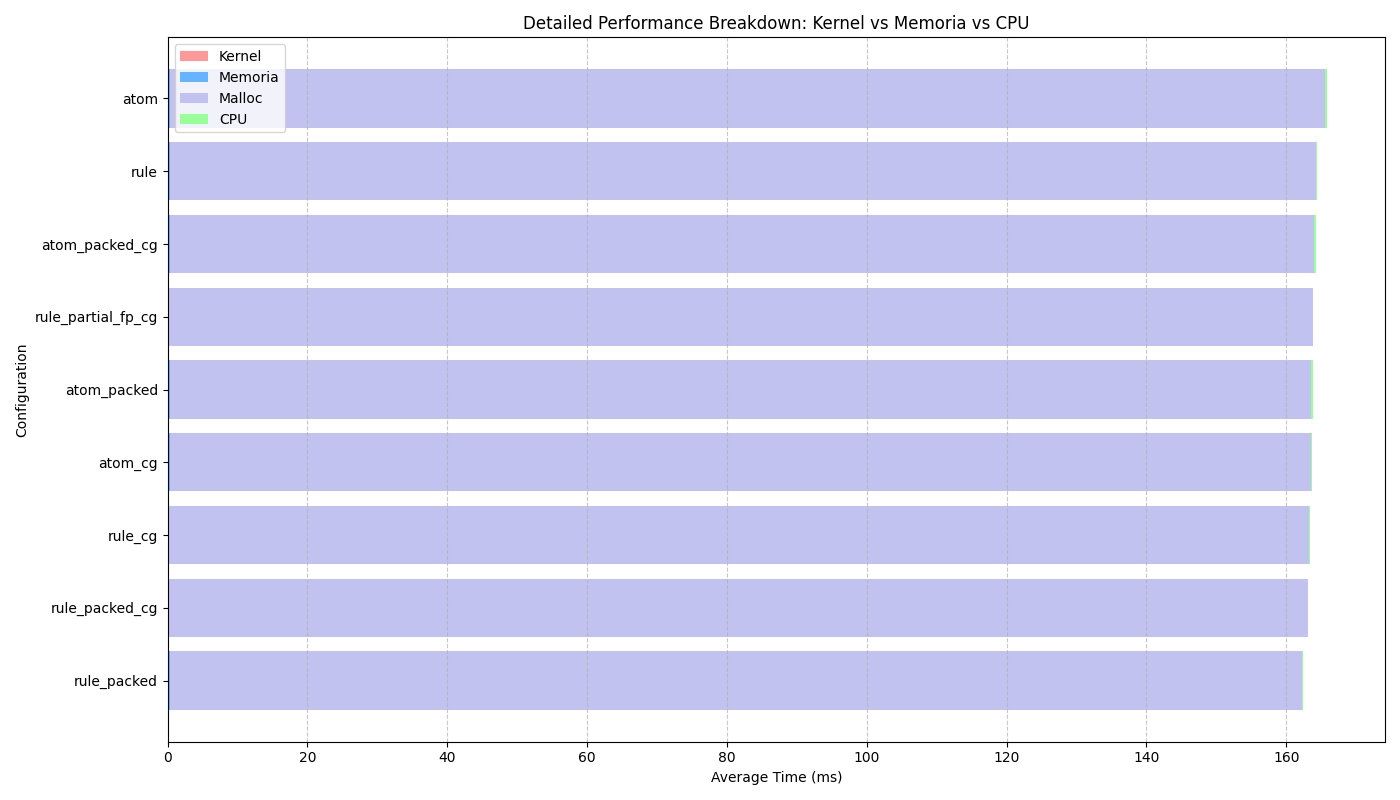
\includegraphics[width=0.85\textwidth]{tests/sudoku/stats/performance_comparison_full.png}
\caption{Confronto del tempo totale (incluso \texttt{cudaMalloc}) tra le nove varianti.}
\end{figure}

\begin{figure}[h]
\centering
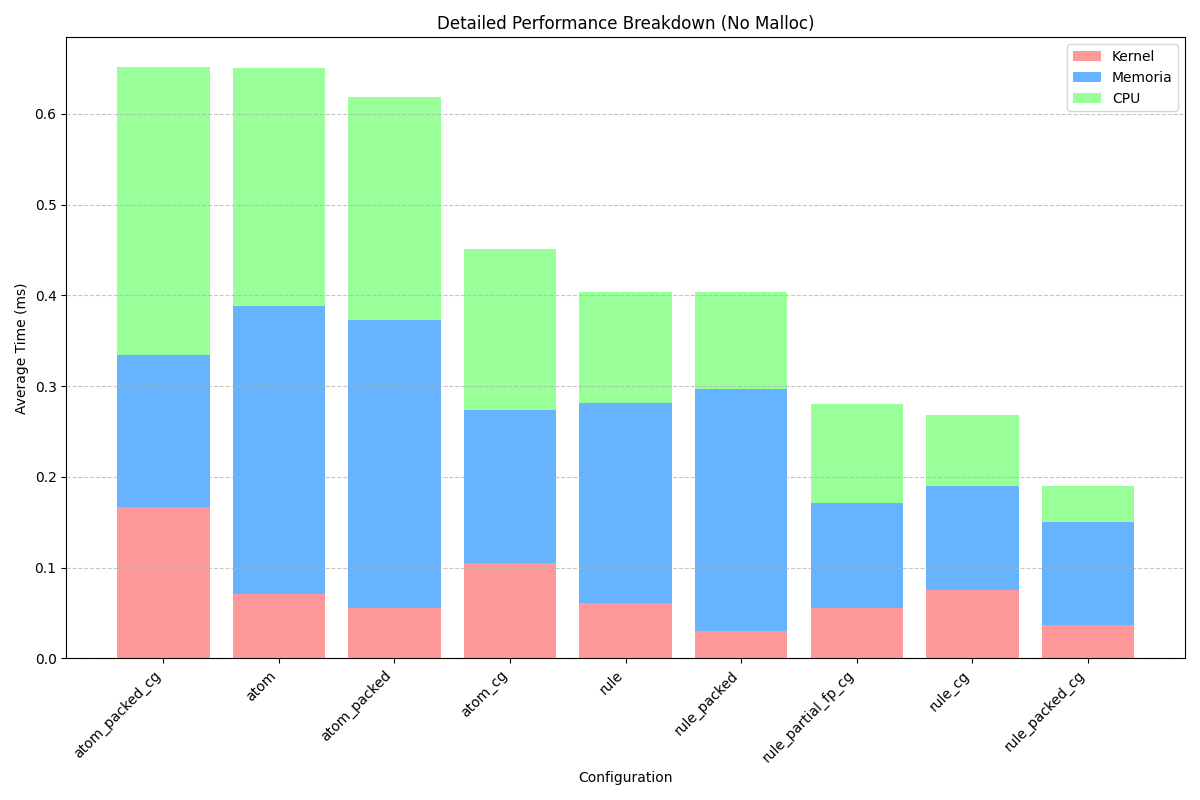
\includegraphics[width=0.85\textwidth]{tests/sudoku/stats/performance_comparison_no_malloc.png}
\caption{Confronto escludendo il tempo di \texttt{cudaMalloc}, per isolare il costo effettivo di kernel e trasferimenti.}
\end{figure}

\subsection{Discussione}

Il primo dato evidente è che, su istanze piccole come il Sudoku $9\times9$, il tempo di
\texttt{cudaMalloc} domina il tempo totale (oltre il 98\% in ogni configurazione): l'allocazione di
memoria sul device ha un costo fisso che non dipende dalla strategia di propagazione, e per istanze
di queste dimensioni satura completamente il confronto se si guarda solo al tempo totale. Il
confronto significativo tra le strategie va quindi fatto sul \emph{tempo di kernel}, dove le
differenze tra le varianti emergono chiaramente (da circa 30\,$\mu$s a oltre 105\,$\mu$s).

Su questa metrica, \texttt{rule\_packed} risulta il più rapido, seguito da \texttt{rule\_packed\_cg}:
il packing a tile, che riduce regole piccole (come quelle del Sudoku, con pochi letterali nel body)
a un singolo warp/tile con riduzione via \texttt{shfl\_down}, si rivela la leva di ottimizzazione più
efficace, più della sincronizzazione globale via cooperative groups. Le due varianti packed restano
le migliori anche guardando il tempo totale (Tabella~\ref{tab:perf}), grazie anche a un tempo di
\texttt{cudaMalloc} leggermente inferiore.

Le varianti \texttt{*\_cg} senza packing (\texttt{rule\_cg}, \texttt{atom\_cg}) mostrano un kernel
time superiore alla baseline non cooperativa corrispondente nel caso \texttt{atom\_cg}, segno che il
costo della sincronizzazione di grid (\texttt{grid.sync()}, eseguita più volte per iterazione) non
viene sempre ripagato dal risparmio sui ri-lanci di kernel, soprattutto quando il numero di
iterazioni a punto fisso è già piccolo, come nel caso del Sudoku.

La variante avanzata \texttt{rule\_partial\_fp\_cg} ottiene un kernel time intermedio
(55\,$\mu$s, sostanzialmente alla pari con \texttt{atom\_packed}), nonostante introduca caching
locale e un ciclo a punto fisso a due livelli pensato per ridurre il traffico su memoria globale: su
istanze piccole come queste, l'overhead di gestione della shared memory dinamica e della copia
iniziale di \texttt{M} nel blocco non viene compensato da un numero di iterazioni sufficientemente
alto da rendere vantaggioso il caching, il cui beneficio è presumibilmente più marcato su istanze
con basi di regole molto più grandi o con molte più iterazioni di punto fisso.

In generale, le varianti \textbf{atom-driven} risultano sistematicamente più lente delle
corrispondenti varianti \textbf{rule-driven} (confrontando \texttt{atom} vs.\ \texttt{rule},
\texttt{atom\_cg} vs.\ \texttt{rule\_cg}, \texttt{atom\_packed} vs.\ \texttt{rule\_packed}): il
costo dell'indirezione tramite le tabelle inverse e della gestione della coda di atomi modificati
supera, su istanze di queste dimensioni, il risparmio di lavoro ridondante che lo schema
atom-driven dovrebbe in teoria offrire rispetto al ricalcolo completo delle somme a ogni iterazione
fatto dalle varianti rule-driven.

\section{Conclusioni}

Tutte le nove varianti CUDA producono lo stesso risultato logico, verificato sia sui test unitari
mirati sia sul benchmark Sudoku confrontando con le soluzioni note: le diverse strategie di
parallelizzazione sono quindi intercambiabili dal punto di vista della correttezza, e si
distinguono solo per le prestazioni.

Sul benchmark utilizzato, il packing a tile (\texttt{rule\_packed}/\texttt{rule\_packed\_cg}) è
risultata la scelta più efficace, più dell'uso di cooperative groups a livello di grid o del
caching locale in shared memory introdotto dalla variante più sofisticata
(\texttt{rule\_partial\_fp\_cg}). Questo è in parte attribuibile alle dimensioni contenute delle
istanze di test (regole con pochi letterali nel body, poche iterazioni di punto fisso necessarie),
che non permettono di amortizzare l'overhead delle tecniche più sofisticate. Anche il costo fisso di
\texttt{cudaMalloc}, dominante sul tempo totale per istanze di queste dimensioni, indica che un
confronto più informativo richiederebbe istanze sensibilmente più grandi, oppure il batching di più
puzzle in un unico lancio di kernel per amortizzare i costi fissi di allocazione e per dare alle
strategie con overhead di sincronizzazione più alto (cooperative groups, caching) margine per
ripagarsi su un numero maggiore di iterazioni utili.

\end{document}
